 \documentclass[oneside,11pt]{article}


\usepackage{soul}
\usepackage{natbib}
\usepackage{hyperref}
\usepackage{graphicx}             
\graphicspath{{./Figuras/}}

\usepackage{makecell}
\usepackage[margin=1.0in]{geometry}
\usepackage{float}                
\usepackage{amsmath}
\usepackage{amscd}
\usepackage{amsfonts}
\usepackage{amssymb}
\usepackage{bbm}
\usepackage{booktabs}
\usepackage{nameref}
\usepackage{multirow}
\usepackage[nokeyprefix]{refstyle}
\usepackage{rotating}
\usepackage{threeparttable}
\usepackage{lscape}
\usepackage{enumerate}
\usepackage{afterpage}
\usepackage{caption}
\usepackage{subcaption}
\usepackage{epstopdf}
\epstopdfDeclareGraphicsRule{.tiff}{png}{.png}{convert #1 \OutputFile}
\AppendGraphicsExtensions{.tiff}

\epstopdfDeclareGraphicsRule{.tif}{png}{.png}{convert #1 \OutputFile}
\AppendGraphicsExtensions{.tif}

\usepackage{tikz}
\usetikzlibrary{shapes.geometric, arrows}
\usetikzlibrary{calc}
\usetikzlibrary{matrix}

\tikzset{ 
    table/.style={
        matrix of nodes,
        row sep=-\pgflinewidth,
        column sep=-\pgflinewidth,
        nodes={
            rectangle,
            draw=black,
            align=center
        },
        minimum height=1.5em,
        text depth=0.5ex,
        text height=2ex,
        nodes in empty cells,
%%
        every even row/.style={
            nodes={fill=gray!20}
        },
        column 1/.style={
            nodes={text width=2em,font=\bfseries}
        },
        row 1/.style={
            nodes={
                fill=black,
                text=white,
                font=\bfseries
            }
        }
    }
}


\usepackage{colortbl}

\newtheorem{theorem}{Theorem}
\newtheorem{claim}[theorem]{Claim}



%%% HELPER CODE FOR DEALING WITH EXTERNAL REFERENCES
\usepackage{xr}
\makeatletter
\newcommand*{\addFileDependency}[1]{
  \typeout{(#1)}
  \@addtofilelist{#1}
  \IfFileExists{#1}{}{\typeout{No file #1.}}
}
\makeatother


\newcommand*{\myexternaldocument}[1]{
    \externaldocument{#1}
    \addFileDependency{#1.tex}
    \addFileDependency{#1.aux}
}

%\myexternaldocument{OA}

%%%%%%%%%%%%%%%%%%%%%%%%%%%%%%%% DOCUMENT
\begin{document}


\section{Heterogeneity}

For a test of heterogeneity we compute the best linear fit of the target estimand using the forest prediction (on held-out data) as well as the mean forest prediction as the sole two regressors. A coefficient of 1 for 'mean.forest.prediction' suggests that the mean forest prediction is correct, whereas a coefficient of 1 for 'differential.forest.prediction' additionally suggests that the forest has captured heterogeneity in the underlying signal.

The p-value of the ‘differential.forest.prediction‘coefficient also acts as an omnibus test the presence of heterogeneity: If the coefficient is significantly greater than 0, then we can reject the null of no heterogeneity.


\begin{table}[H]
\caption{}
\label{}
\begin{center}
\scriptsize{% Table generated by Excel2LaTeX from sheet 'test_calibration'
\begin{tabular}{lrr}
\multicolumn{3}{c}{Test calibration} \\
\midrule
      & \multicolumn{2}{c}{APR BVC} \\
\midrule
\midrule
      & \multicolumn{1}{l}{estimate} & \multicolumn{1}{l}{p-value} \\
\cmidrule{2-3}mean.forest.prediction & 0.99  & 4.67055E-14 \\
differential.forest.prediction & 0.961 & 3.30688E-15 \\
\midrule
      & \multicolumn{2}{c}{APR BVC + survey variables} \\
\midrule
\midrule
      & \multicolumn{1}{l}{estimate} & \multicolumn{1}{l}{p-value} \\
\cmidrule{2-3}mean.forest.prediction & 1.001 & 1.03503E-17 \\
differential.forest.prediction & 1.256 & 1.86116E-09 \\
\midrule
      & \multicolumn{2}{c}{Recovery BVC} \\
\midrule
\midrule
      & \multicolumn{1}{l}{estimate} & \multicolumn{1}{l}{p-value} \\
\cmidrule{2-3}mean.forest.prediction & 0.996 & 7.91647E-11 \\
differential.forest.prediction & 0.981 & 1.80631E-15 \\
\midrule
      & \multicolumn{2}{c}{Recovery BVC + survey variables} \\
\midrule
\midrule
      & \multicolumn{1}{l}{estimate} & \multicolumn{1}{l}{p-value} \\
\cmidrule{2-3}mean.forest.prediction & 1.01  & 2.72902E-15 \\
differential.forest.prediction & 1.1   & 5.71608E-06 \\
\bottomrule
\bottomrule
\end{tabular}%
}
\end{center}

\end{table}


Many tests for heterogeneity:


\cite{a3}  use of a heuristic support-vector-machine method with lasso penalization for classification of heterogeneous treatments into positive and negative ones

\begin{thebibliography}{2}

\bibitem{a1} Generic Machine Learning Inference on Heterogenous Treatment Effects in Randomized Experiments. Chernozhukov, Victor, Mert Demirer, Esther Duflo, and Ivan Fernandez-Val



\bibitem{a3} Estimating Treatment Effect Heterogeneity In Randomized Program Evaluation. Kosuke Imai, Ratkovic

\bibitem{a4} Testing for Essential Heterogeneity. Heckman
\bibitem{a12} Nonparametric  Tests  for Treatment  Effect  Heterogeneity. Crump et.al

\bibitem{a5} Treatment Effect Heterogeneity In Theory And Practice . Angrist

\bibitem{a6} Evaluating Treatment Prioritization Rules via Rank-Weighted Average Treatment Effects. Wager et. al.

\bibitem{a2} Brand, J. E., Y. Xie (2010). Who Benefits Most From College?Evidence for Negative Selection in Heterogeneous Economic Returns to Higher Education

\end{thebibliography}

\subsection{Some points}

\begin{itemize}
    \item Doubts of how to construct a sharp bound for the variance of a treatment effect of Heckman et al. (1997). $->$ This in order to argue there is heterogeneity.
    
    \item I am currently trying to implement Empirical deconvolution of Heckman et al. (1997).
\end{itemize}




% Table generated by Excel2LaTeX from sheet 'grf_pro_2_apr_ate'
\begin{tabular}{rrl}
\multicolumn{1}{l}{beta} & \multicolumn{1}{l}{se} & target\_sample \\
-38.0631 & 3.793024 & all \\
-37.2934 & 4.438196 & overlap \\
-34.4718 & 4.344636 & treated \\
-41.0618 & 4.279213 & control \\
\end{tabular}%

\newpage

\section{Bounds}


\begin{table}[H]
\caption{Gains for choosers versus gains from non-choosers (ToT \& TuT)}
\label{tot_tut}
\begin{center}
\scriptsize{% Table generated by Excel2LaTeX from sheet 'tot_tut_reg'
\begin{tabular}{lccccccccccc}
\toprule
      & \multicolumn{2}{c}{APR} &       & \multicolumn{2}{c}{Recovery} &       & \multicolumn{2}{c}{Financial Benefit/loan} &       & \multicolumn{2}{c}{Recovery or No payment} \\
\cmidrule{2-3}\cmidrule{5-6}\cmidrule{8-9}\cmidrule{11-12}      & (1)   & (2)   &       & (3)   & (4)   &       & (5)   & (6)   &       & (7)   & (8) \\
\midrule
\midrule
Forced commitment & 32.5*** & 39.7*** &       & 0.11*** & 0.12*** &       & 0.061*** & 0.074*** &       & 0.11*** & 0.13*** \\
      & (6.80) & (6.41) &       & (0.023) & (0.022) &       & (0.013) & (0.012) &       & (0.020) & (0.020) \\
Choice commitment & -7.50 & -1.52 &       & -0.0062 & 0.0021 &       & -0.015 & -0.0036 &       & -0.017 & 0.0053 \\
      & (8.21) & (6.43) &       & (0.021) & (0.019) &       & (0.016) & (0.012) &       & (0.025) & (0.018) \\
      &       &       &       &       &       &       &       &       &       &       &  \\
\midrule
\rowcolor[rgb]{ .949,  .949,  .949} ToT   & -74.5 & -15.1 &       & -0.061 & 0.020 &       & -0.15 & -0.036 &       & -0.17 & 0.053 \\
Clustered p-value & 0.36  & 0.81  &       & 0.77  & 0.91  &       & 0.34  & 0.77  &       & 0.48  & 0.77 \\
\rowcolor[rgb]{ .949,  .949,  .949} TuT   & 44.5  & 45.9  &       & 0.12  & 0.13  &       & 0.08  & 0.09  &       & 0.14  & 0.14 \\
Clustered p-value & 1.50E-06 & 6.50E-08 &       & 1.80E-06 & 4.40E-07 &       & 2.00E-06 & 1.00E-07 &       & 3.80E-08 & 1.20E-08 \\
\rowcolor[rgb]{ .949,  .949,  .949} ToT-TuT & -119.0 & -60.9 &       & -0.19 & -0.11 &       & -0.23 & -0.12 &       & -0.31 & -0.085 \\
F clustered p-value & 0.088 & 0.19  &       & 0.20  & 0.30  &       & 0.082 & 0.18  &       & 0.12  & 0.33 \\
Bootstrap (normal) p-val & 0.100 & 0.24  &       & 0.20  & 0.32  &       & 0.091 & 0.22  &       & 0.12  & 0.38 \\
Bootstrap (percentile) p-val & 0.089 & 0.24  &       & 0.19  & 0.33  &       & 0.079 & 0.21  &       & 0.12  & 0.38 \\
RI p-val & 0.11  & 0.24  &       & 0.24  & 0.35  &       & 0.11  & 0.24  &       & 0.14  & 0.38 \\
\midrule
      &       &       &       &       &       &       &       &       &       &       &  \\
\midrule
Observations & 8519  & 8519  &       & 8519  & 8519  &       & 8519  & 8519  &       & 8519  & 8519 \\
R-squared & 0.014 & 0.038 &       & 0.010 & 0.022 &       & 0.013 & 0.038 &       & 0.016 & 0.042 \\
Control Mean & \multicolumn{2}{c}{-248.7} &       & \multicolumn{2}{c}{0.44} &       & \multicolumn{2}{c}{1.45} &       & \multicolumn{2}{c}{0.75} \\
Controls &       & \checkmark &       &       & \checkmark &       &       & \checkmark &       &       & \checkmark \\
\bottomrule
\bottomrule
\end{tabular}%
}
\end{center}
 \scriptsize This table shows estimates of the ToT and the TuT with an IV-LATE framework. The ToT is computed as the usual LATE with one-sided non-compliance between the choice and control arm, and the TuT is the LATE on non-compliers. 
%\textit{Do file: } \texttt{tot\_tut\_reg.do}
\end{table}

The Huber \& Mellace (2015) bounds for the TOT \& TUT APR are respectively:
$[-481.8, 483.7]$ , $[-17.9, 90.6]$. \\

\subsection{Question:}

\textit{IV validity implies that the mean outcome of the treated receiving the instrument is equal to that of the treated not receiving the instrument. This can be easily tested by difference-of-means tests. An analogous result holds for the never takers and the compliers under non treatment}


\textbf{Isn't this then a test for the above?}



\begin{figure}[H]
     \caption{Exclusion restriction}
     \label{exclusion_restriction}
    \begin{center}
    \begin{subfigure}{0.6\textwidth}
        \centering
        \includegraphics[width=\textwidth]{Figuras/exclusion_restriction.pdf}
    \end{subfigure}
    \end{center}
    \scriptsize This figure serves as a test for the exclusion restriction in the point identification for the ToT and the TuT. It shows the effect on the effective cost/loan ratio for the forced-fee arm and the choice arm, together with the decomposition of the choosers and non-choosers. Note that a) being forced into the treatment (Forced fee) has the same effect as choosing it (Choosers), and b) not choosing the treatment (Non chooser) has no effect with respect to the control.
    
          %\footnotesize{ \textit{Do file: }  \texttt{exclusion\_restriction.do}}
\end{figure}




The next figure implements the  Fan \& Park (2010) bounds for the TE


\begin{figure}[H]
    \caption{Fan \& Park bounds}
    \label{fan_park_bounds}
    \begin{center}

    \begin{subfigure}{0.475\textwidth}
        \caption{APR}
        \centering
        \includegraphics[width=\textwidth]{Figuras/fan_park_bounds_apr.pdf}
    \end{subfigure}
    \begin{subfigure}{0.475\textwidth}
        \caption{Financial Cost}
        \centering
        \includegraphics[width=\textwidth]{Figuras/fan_park_bounds_fc_admin.pdf}
    \end{subfigure}
    \begin{subfigure}{0.475\textwidth}
        \caption{Recovery}
        \centering
        \includegraphics[width=\textwidth]{Figuras/fan_park_bounds_des_c.pdf}
    \end{subfigure}    
    \end{center}
\end{figure}


The next is a figure for the bounds for the QTE


\begin{figure}[H]
    \caption{}
    \label{}
    \begin{center}

    \begin{subfigure}{0.475\textwidth}
        \caption{APR}
        \centering
        \includegraphics[width=\textwidth]{Figuras/fan_park_qbounds_apr.pdf}
    \end{subfigure}
    \begin{subfigure}{0.475\textwidth}
        \caption{Financial Cost}
        \centering
        \includegraphics[width=\textwidth]{Figuras/fan_park_qbounds_fc_admin.pdf}
    \end{subfigure}

    \end{center}
\end{figure}

\subsection{Question:}

\textbf{Should we, and more importantly, can we do this for the TOT \& TUT?}



\section{Machine Learning exercises}

\subsection{First ML exercise}



\begin{figure}[H]
    \caption{Choice of contracts and treatment effects using TOT \& TUT}
    \label{choose_wrong}
    \begin{center}
        \begin{subfigure}{0.45\textwidth}
        \caption{Mistakes in choice arm}
        \centering
        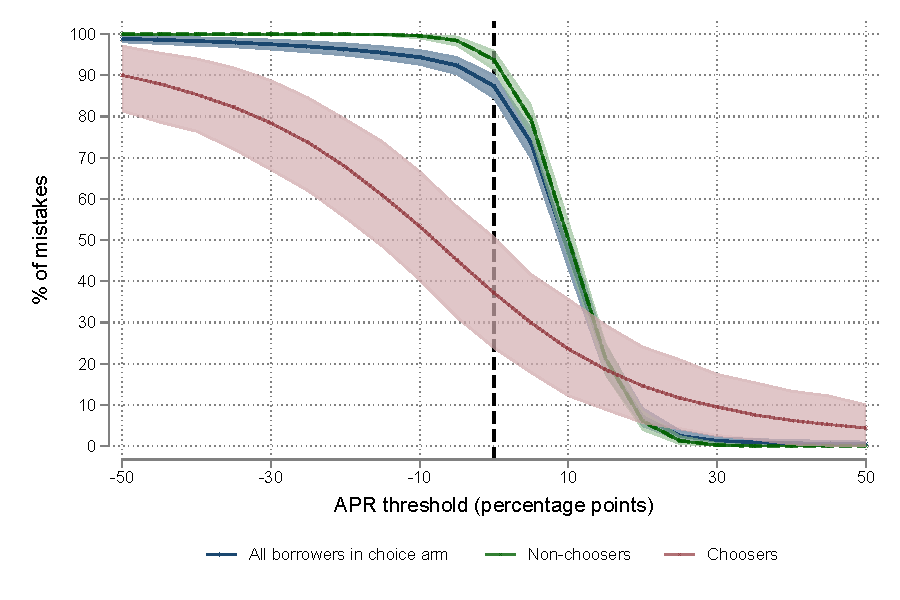
\includegraphics[width=\textwidth]{Figuras/line_cw_apr_tot_tut.pdf}
        
    \end{subfigure}
        \begin{subfigure}{0.45\textwidth}
        \caption{Financial value of mistake}
        \centering
        \includegraphics[width=\textwidth]{Figuras/money_cw_apr_tot_tut.pdf}
 \end{subfigure}
    \bigskip
        
    \end{center}
    
\end{figure}

\subsection{Second ML exercise}




\begin{figure}[H]
    \caption{}
    \label{choose_wrong}
    \begin{center}
        \begin{subfigure}{0.45\textwidth}
        \caption{Gradient Boosting}
        \centering
        \includegraphics[width=\textwidth]{Figuras/ps_te_apr.pdf}
        
    \end{subfigure}
        \begin{subfigure}{0.45\textwidth}
        \caption{KNN}
        \centering
        \includegraphics[width=\textwidth]{Figuras/ps_te_apr1.pdf}
 \end{subfigure}
    \bigskip
        
    \end{center}
    
\end{figure}

\subsubsection{Question:}
\textit{As in the previous exercise, I think it might be worth trying to say something about the conditional TUT without invoking Assumption 3, and I think we can do this using a conditional LATE, given our design.}


\newpage
\clearpage

\begin{landscape}
\begin{table}[H]
\caption{}
\label{}
\begin{center}
\resizebox{1.5\textwidth}{!}{
\scriptsize{% Table generated by Excel2LaTeX from sheet 'tot_tut_se'
\begin{tabular}{lcccccccccccccccccccccccccc}
\toprule
      & \multicolumn{26}{c}{APR} \\
\midrule
      & \multicolumn{11}{c}{ToT}                                                              &       & \multicolumn{11}{c}{TuT}                                                              &       & \multicolumn{2}{c}{ToT \& TuT} \\
\cmidrule{2-12}\cmidrule{14-24}\cmidrule{26-27}      & \multicolumn{2}{c}{Single LATE} &       & \multicolumn{2}{c}{LATE + ATE} &       & \multicolumn{2}{c}{Plug-in estimator} &       & \multicolumn{2}{c}{GMM} &       & \multicolumn{2}{c}{Single LATE} &       & \multicolumn{2}{c}{LATE + ATE} &       & \multicolumn{2}{c}{Plug-in estimator} &       & \multicolumn{2}{c}{GMM} &       & \multicolumn{2}{c}{Stacked GMM} \\
\cmidrule{2-3}\cmidrule{5-6}\cmidrule{8-9}\cmidrule{11-12}\cmidrule{14-15}\cmidrule{17-18}\cmidrule{20-21}\cmidrule{23-24}\cmidrule{26-27}      & (1)   & (2)   &       & (3)   & (4)   &       & (5)   & (6)   &       & (7)   & (8)   &       & (9)   & (10)  &       & (11)  & (12)  &       & (13)  & (14)  &       & (15)  & (16)  &       & (17)  & (18) \\
\midrule
\midrule
ATE (Forced commitment) &       &       &       & 32.8*** & 40.1*** &       & 32.8*** & 40.0*** &       & 32.8*** & 40.1*** &       &       &       &       & 32.8*** & 39.7*** &       & 32.8*** & 40.0*** &       & 32.8*** & 43.2*** &       & 32.8*** & 43.5*** \\
      &       &       &       & (6.79) & (6.26) &       & (6.81) & (6.40) &       & (6.79) & (6.26) &       &       &       &       & (6.79) & (6.31) &       & (6.81) & (6.40) &       & (6.79) & (6.40) &       & (6.79) & (6.41) \\
ATE (Forced choice) &       &       &       &       &       &       & -7.51 & -1.53 &       &       &       &       &       &       &       &       &       &       & -7.51 & -1.53 &       &       &       &       &       &  \\
      &       &       &       &       &       &       & (8.20) & (6.42) &       &       &       &       &       &       &       &       &       &       & (8.20) & (6.42) &       &       &       &       &       &  \\
ToT   & -74.6 & 11.0  &       & -74.6 & -14.9 &       & -74.6 & -15.2 &       & -74.6 & -14.9 &       &       &       &       &       &       &       &       &       &       &       &       &       & -74.6 & -52.4 \\
      & (84.4) & (58.4) &       & (84.4) & (62.4) &       & (81.4) & (63.8) &       & (84.4) & (62.4) &       &       &       &       &       &       &       &       &       &       &       &       &       & (84.4) & (62.7) \\
TuT   &       &       &       &       &       &       &       &       &       &       &       &       & 44.8*** & 44.8*** &       & 44.8*** & 45.9*** &       & 44.8*** & 46.2*** &       & 44.8*** & 49.3*** &       & 44.8*** & 49.6*** \\
      &       &       &       &       &       &       &       &       &       &       &       &       & (8.84) & (8.01) &       & (8.84) & (8.05) &       & (9.02) & (8.24) &       & (8.84) & (8.06) &       & (8.84) & (8.06) \\
Control Mean $\mathbb{E}[Y_0]$ & -249.0*** & -220.4*** &       & -249.0*** & -223.4*** &       & -249.0*** & -225.1*** &       & -249.0*** & -112.8*** &       & -261.0*** & -239.6*** &       & -216.2*** & -190.7*** &       & -249.0*** & -225.1*** &       &       &       &       & -249.0*** & -38.9** \\
      & (4.87) & (16.9) &       & (4.87) & (15.3) &       & (4.88) & (10.8) &       & (4.87) & (15.3) &       & (7.13) & (12.0) &       & (4.73) & (10.6) &       & (4.88) & (10.8) &       &       &       &       & (4.87) & (16.2) \\
Treated Mean $\mathbb{E}[Y_1]$ &       &       &       &       &       &       &       &       &       &       &       &       &       &       &       &       &       &       &       &       &       & -216.2*** & -34.0*** &       & -216.2*** & -33.6*** \\
      &       &       &       &       &       &       &       &       &       &       &       &       &       &       &       &       &       &       &       &       &       & (4.73) & (11.4) &       & (4.73) & (11.5) \\
      &       &       &       &       &       &       &       &       &       &       &       &       &       &       &       &       &       &       &       &       &       &       &       &       &       &  \\
\midrule
Observations & 6035  & 6035  &       & 8519  & 8519  &       & 8519  & 8519  &       & 8519  & 8519  &       & 5919  & 5919  &       & 8519  & 8519  &       & 8519  & 8519  &       & 8519  & 8519  &       & 8519  & 8519 \\
R-squared & .     & 0.043 &       & .     & 0.035 &       & 0.014 & 0.038 &       &       &       &       & 0.028 & 0.052 &       & 0.021 & 0.044 &       & 0.014 & 0.038 &       &       &       &       &       &  \\
Controls &       & \checkmark &       &       & \checkmark &       &       & \checkmark &       &       & \checkmark &       &       & \checkmark &       &       & \checkmark &       &       & \checkmark &       &       & \checkmark &       &       & \checkmark \\
\midrule
$H_0 : \operatorname{ATE}-\operatorname{ToT} = 0$ &       &       &       & 0.19  & 0.37  &       &       &       &       & 0.19  & 0.37  &       &       &       &       &       &       &       &       &       &       &       &       &       & 0.19  & 0.14 \\
$H_0 : \operatorname{ATE}-\operatorname{TuT} = 0$ &       &       &       &       &       &       &       &       &       &       &       &       &       &       &       & 0.16  & 0.36  &       &       &       &       & 0.16  & 0.37  &       & 0.16  & 0.37 \\
$H_0 : \operatorname{TuT}-\operatorname{ToT} = 0$ &       &       &       &       &       &       &       &       &       &       &       &       &       &       &       &       &       &       &       &       &       &       &       &       & 0.19  & 0.13 \\
$H_0 : \operatorname{TuT}-\operatorname{ToT} \geq 0$ &       &       &       &       &       &       &       &       &       &       &       &       &       &       &       &       &       &       &       &       &       &       &       &       & 0.91  & 0.065 \\
\bottomrule
\bottomrule
\end{tabular}%
}
}
\end{center}

\end{table}

\end{landscape}

\end{document}
